\documentclass{memoir}

%% from https://github.com/hadley/r-pkgs/blob/master/book/r-packages.tex
\usepackage[T1]{fontenc}
\usepackage{lmodern}
\usepackage{amssymb,amsmath}
\usepackage{upquote}

\usepackage{fontspec}
\usepackage{xltxtra,xunicode}
\defaultfontfeatures{Mapping=tex-text,Scale=MatchLowercase}
\setmonofont[Mapping=tex-ansi]{Inconsolata}

% Taken from pandoc x.md -o test.tex --standalone
\usepackage{color}
\usepackage{fancyvrb}
\newcommand{\VerbBar}{|}
\newcommand{\VERB}{\Verb[commandchars=\\\{\}]}
\DefineVerbatimEnvironment{Highlighting}{Verbatim}{commandchars=\\\{\}}
\newenvironment{Shaded}{}{}
\newcommand{\KeywordTok} [1]{\textcolor[rgb]{0.00,0.44,0.13}{{#1}}}
\newcommand{\DataTypeTok}[1]{\textcolor[rgb]{0.56,0.13,0.00}{{#1}}}
\newcommand{\DecValTok}  [1]{\textcolor[rgb]{0.25,0.63,0.44}{{#1}}}
\newcommand{\BaseNTok}   [1]{\textcolor[rgb]{0.25,0.63,0.44}{{#1}}}
\newcommand{\FloatTok}   [1]{\textcolor[rgb]{0.25,0.63,0.44}{{#1}}}
\newcommand{\CharTok}    [1]{\textcolor[rgb]{0.25,0.44,0.63}{{#1}}}
\newcommand{\StringTok}  [1]{\textcolor[rgb]{0.25,0.44,0.63}{{#1}}}
\newcommand{\CommentTok} [1]{\textcolor[rgb]{0.38,0.63,0.69}{{#1}}}
\newcommand{\OtherTok}   [1]{\textcolor[rgb]{0.00,0.44,0.13}{{#1}}}
\newcommand{\AlertTok}   [1]{\textcolor[rgb]{1.00,0.00,0.00}{{#1}}}
\newcommand{\FunctionTok}[1]{\textcolor[rgb]{0.02,0.16,0.49}{{#1}}}
\newcommand{\ErrorTok}   [1]{\textcolor[rgb]{1.00,0.00,0.00}{{#1}}}
\newcommand{\NormalTok}  [1]{{#1}}

\usepackage{longtable}
\usepackage{booktabs}
\usepackage{graphicx}
\usepackage{emptypage}
\raggedbottom

\usepackage[hyphens]{url}
\usepackage[setpagesize=false, % page size defined by xetex
            unicode=false, % unicode breaks when used with xetex
            xetex,
			hidelinks]{hyperref}

% Place links as footnotes
\renewcommand{\href}[2]{#2 (\url{#1})}
% Use ref for internal links
\renewcommand{\hyperref}[2][???]{\autoref{#1}}
\def\chapterautorefname{Chapter}
\def\sectionautorefname{Section}
\def\subsectionautorefname{Section}
\def\subsubsectionautorefname{Section}

\setlength{\parindent}{0pt}
\setlength{\parskip}{6pt plus 2pt minus 1pt}
\setlength{\emergencystretch}{3em}  % prevent overfull lines
\vbadness=10000 % suppress underfull \vbox
\hbadness=10000 % suppress underfull \vbox
\hfuzz=1pt

%% BEGIN TITLE PAGE

\makeatletter
\def\maketitle{%
  \null
  \thispagestyle{empty}%
  \vfill
  \begin{center}\leavevmode
    \normalfont
    {\LARGE\raggedleft \@author\par}%
    \hrulefill\par
    {\huge\raggedright \@title\par}%
    \vskip 1cm
%    {\Large \@date\par}%
  \end{center}%
  \vfill
  \null
  \cleardoublepage
  }
\makeatother
\author{Author's name}
\title{Book's title}
\date{}



\makeindex

\begin{document}

\frontmatter

\maketitle


% \listoftables
\tableofcontents

\mainmatter

%% edit the below list by hand to get the chapters in order

\chapter{Heading of Test Chapter 1}\label{testchapterone}

This is a chapter of the book for testing. It has code to be executed,
and citations to be processed. The code produces a plot (Figure 1.1).

We are testing to see if a bib file and a csl can be used with the
bookdown package to produce chapters that have a reference list at the
end.

\begin{Shaded}
\begin{Highlighting}[]
\KeywordTok{plot}\NormalTok{(}\KeywordTok{rnorm}\NormalTok{(}\DecValTok{1000}\NormalTok{))}
\end{Highlighting}
\end{Shaded}

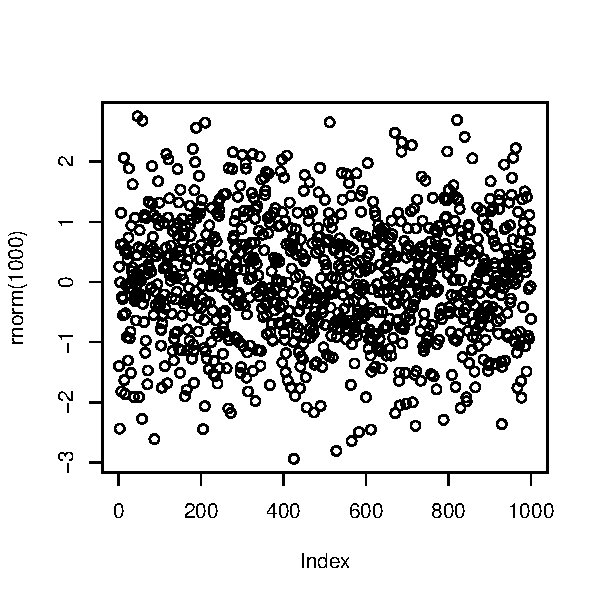
\includegraphics{figures/simple_plot-1.pdf}

Figure 1.1: Plot of 100 values randomly sampled from a normal
distribution.

Some of the best recent books on R include Hadley Wickham's `Advanced R'
(2014). He also has a very useful book on R packages (Wickham, 2015).

\section*{References}
\addcontentsline{toc}{section}{References}

Wickham, H. (2014). \emph{Advanced R}. CRC Press.

Wickham, H. (2015). \emph{R packages}. O'Reilly Media, Inc.

\chapter{Heading of Test Chapter 2}\label{testchaptertwo}

This is another chapter of the book.

\begin{Shaded}
\begin{Highlighting}[]
\KeywordTok{plot}\NormalTok{(faithful, }\DataTypeTok{col =} \StringTok{"blue"}\NormalTok{, }\DataTypeTok{main =} \StringTok{"Eruptions of Old Faithful"}\NormalTok{)}
\end{Highlighting}
\end{Shaded}

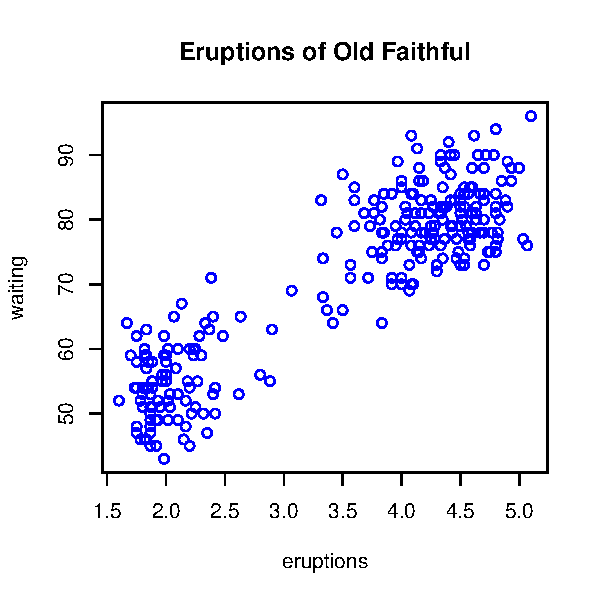
\includegraphics{figures/old_faithful-1.pdf}

Figure 2.1: Eruptions of Old Faithful

This is a \emph{very} basic plot (Figure 2.1). But it's easy to make
very elegant and useful visuaisations with R, thanks to the numerous
accessible books on the topic (Chang, 2012; Murrell, 2011; Wickham,
2009)

\section*{References}
\addcontentsline{toc}{section}{References}

Chang, W. (2012). \emph{R graphics cookbook}. `` O'Reilly Media, Inc.''

Murrell, P. (2011). \emph{R graphics}. CRC Press.

Wickham, H. (2009). \emph{Ggplot2: Elegant graphics for data analysis}.
Springer Science \& Business Media.


\end{document}
